\section{The Control Plane}

\begin{frame}[noframenumbering, plain]
    \sectionpage
\end{frame}

% He must wander
\togglefalse{DINOSAUR}
\begin{frame}{Fine Tuning Inputs- The Control Plane}
    \begin{itemize}
        \item vf3's data plane forms one of the fastest syntactic engines, it's also the only
        engine with dedicated infrastructure for generalized advanced state machines.
        \item Under the hood, all of vf3's data plane is represented by graphs; thus, the engine's
        controls manifest as {\color{themetitle}\textit{graph edits}}. 
        \item Input machinery, the program harness, and controls coalesce into a
        {\color{themetitle}\textit{campaign}}.
    \end{itemize}

    \vspace{1.33cm}
    \begin{tikzpicture}[remember picture, overlay]
        \node[draw=none] (offset) at (2cm, 0.25cm) {};
        \AnimateNode{2-}{draw=none} (dinosaur)  at ($(offset) + (0, 0)$)
            {
\includegraphics[width=0.07\textwidth]{images/dino.png}};
        \AnimateNode{2-}{draw=none} (qmark) at ($(dinosaur) + (0cm, 0.65cm)$)
            {\large{?}};
        \AnimateNode{3-}{draw=none} (robot) at ($(dinosaur) + (3.5cm, 0)$)
            {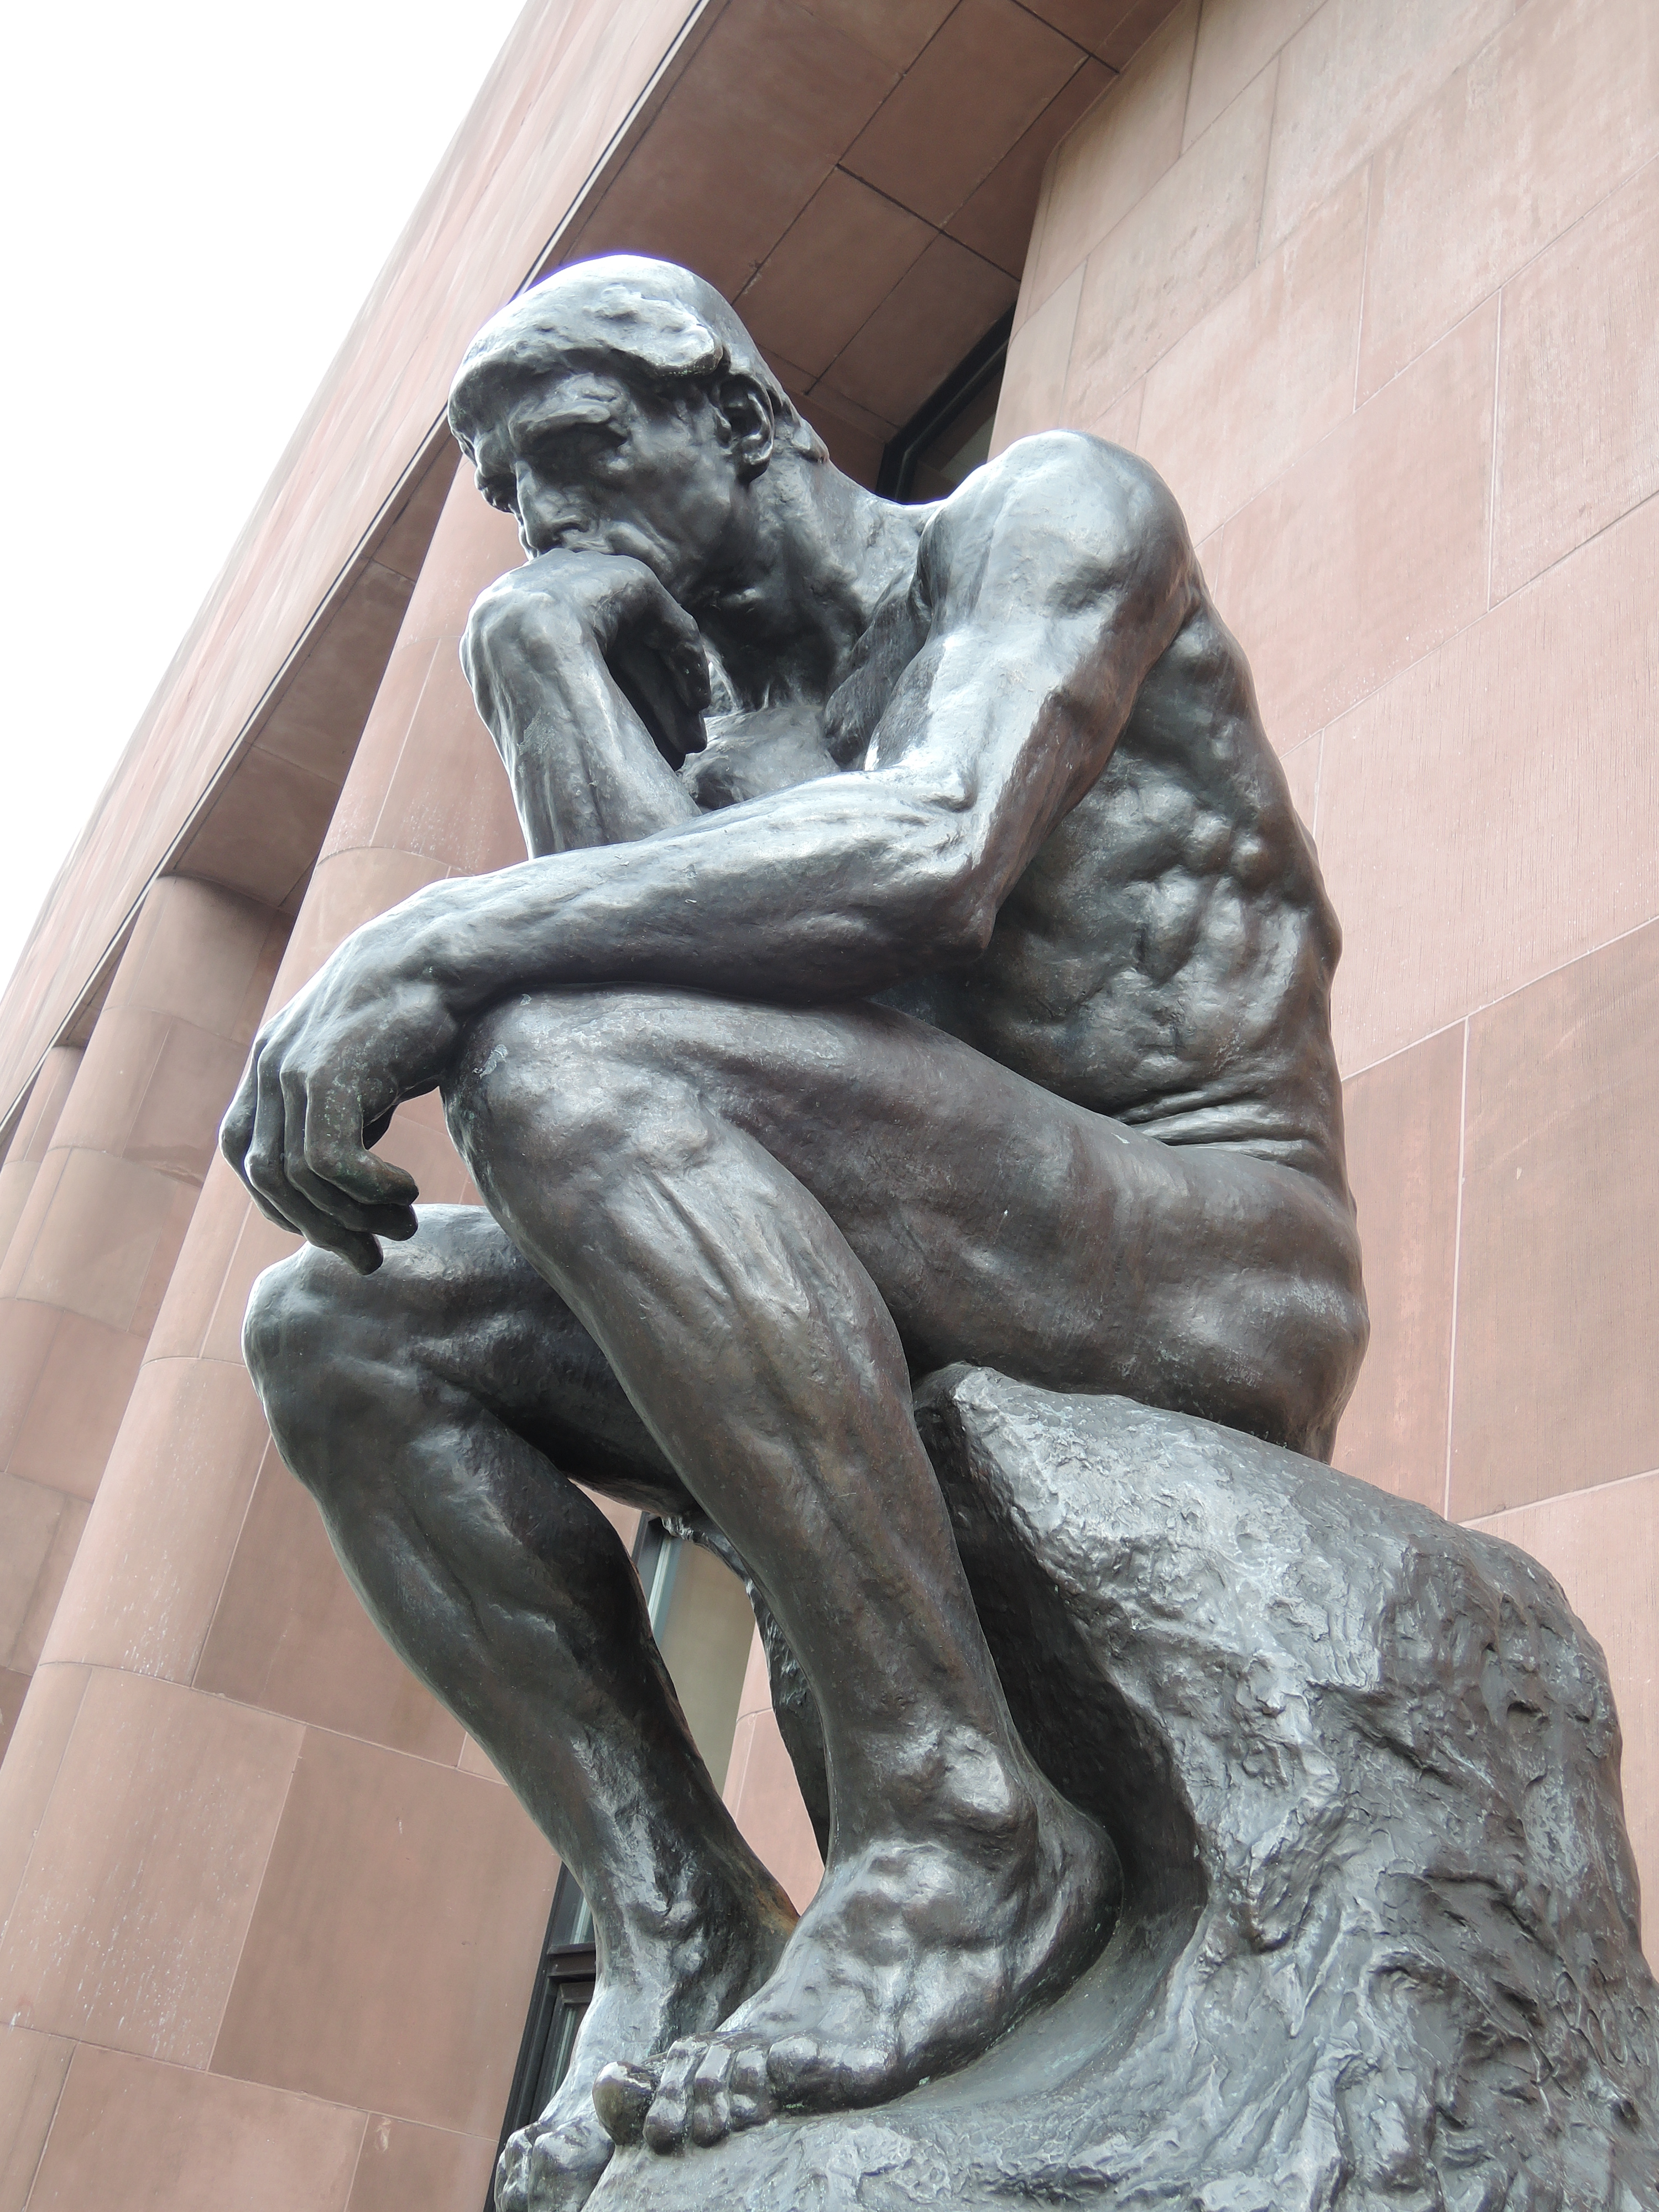
\includegraphics[width=0.12\textwidth]{images/thinker.jpeg}};

        % Small matrix
        \AnimateNode{4-}{draw=none, inner sep=0pt} (program) at ($(robot) + (3.5cm, 0.5cm)$) {\scriptsize 1 0 1 0 0 1};
        \AnimateNode{4-}{draw=none, inner sep=0pt} (program2) at ($(robot) + (3.5cm, 0.2cm)$) {\scriptsize 1 0 1 0 1 0};
        \AnimateNode{4-}{draw=none, inner sep=0pt} (program3) at ($(robot) + (3.5cm, -0.1cm)$) {\scriptsize 0 0 1 1 0 0};
        \AnimateNode{4-}{draw=none, inner sep=0pt} (program4) at ($(robot) + (3.5cm, -0.4cm)$) {\scriptsize 1 0 1 1 1 0};

        % Graph edits
        \AnimateNode{5-}{circle, inner sep=3pt, fill=themefont} (n1) at
            ($(program) + (2.9cm, 0cm)$) {};
        \AnimateNode{5-}{circle, inner sep=3pt, fill=themefont} (n2) at
            ($(n1) + (1cm, -0.33cm)$) {};
        \AnimateNode{5-}{circle, inner sep=3pt, fill=themestrong} (n3) at
            ($(n1) + (1.5cm, -1cm)$) {};
        \AnimateNode{5-}{circle, inner sep=3pt, fill=themeaccent} (n4) at
            ($(n1) + (0cm, -0.65cm)$) {};
        \AnimateNode{5-}{circle, inner sep=3pt, fill=themefont} (n5) at
            ($(n1) + (0.45cm, -1cm)$) {};
        \AnimateNode{5-}{circle, inner sep=3pt, fill=themetitle} (n6) at
            ($(n1) + (1.25cm, 0.25cm)$) {};

        \AnimateDraw{5-}{-, themefont} (n1) -- (n2);
        \AnimateDraw{5-}{-, themefont} (n1) -- (n4);
        \AnimateDraw{5-}{-, themefont} (n2) -- (n3);
        \AnimateDraw{5-}{-, themefont} (n4) -- (n5);
        \AnimateDraw{5-}{-, themefont} (n2) -- (n6);

        % text labels
        \AnimateNode{2-}{draw=none} (dlabel) at ($(dinosaur) + (0cm, -0.9cm)$)
            {\footnotesize{1. Fuzzer stuck}};

        \AnimateNode{3-}{draw=none} (rlabel) at ($(robot) + (0cm, -1.6cm)$)
            {\footnotesize{2. Ask large language friend}};

        \AnimateNode{4-}{draw=none} (plabel) at ($(program) + (0cm, -1.5cm)$)
            {\footnotesize{3. Gather context}};

        \AnimateNode{5-}{draw=none} (glabel) at ($(n1) + (0.75cm, -1.5cm)$)
            {\footnotesize{4. Make graph edits}};

        % Accented arrows
        \AnimateDraw{3-}{->, themeaccent} (dinosaur.east) --
            ($(robot.west) + (-0.2cm, 0cm)$);
        \AnimateDraw{4-}{->, themeaccent}
            ($(dinosaur.east) + (4.0cm, 0cm)$)  --
            ($(dinosaur.east) + (5.4cm, 0cm)$);
        \AnimateDraw{5-}{->, themeaccent}
            ($(dinosaur.east) + (7.35cm, 0cm)$)  --
            ($(dinosaur.east) + (8.75cm, 0cm)$);

    \end{tikzpicture}
    \vspace{0.33cm}
\end{frame}
\toggletrue{DINOSAUR}

\begin{frame}{When do I click the AI button?}
    AI is awesome, but it's really really slow. It can also be really expensive. We can
    mathematically determine ideal conditions to solicit help from AI.
    \begin{equation*}
        D_{KL}(P || Q) = \sum_{x \in X} P(x) ln(\frac{P(x)}{Q(x)})
    \end{equation*}
    \begin{itemize}
        \item This equation is called Kullback-Leibler (KL) divergence, it measures how
        far one probability distribution \textit{Q} is from a target distribution \textit{P}. 
        \item In our case, if the fuzzer how no idea what it's doing, each input we
        process will have uniform or near-uniform response. P(x) will look like 1/N for N inputs.
    \end{itemize}
\end{frame}

\begin{frame}{Prompting and Gathering Context}
    \begin{itemize}
        \item vf3 routes its API calls through \themeref{https://github.com/BerriAI/litellm}{litellm},
        providing the model context via \textit{\color{themetitle}tool calls}.
        \begin{multicols}{2}
            \begin{itemize}
                \item State \& grammar info
                \item Crash reports
                \item Coverage data
                \item Input history
            \end{itemize}
        \end{multicols}
    \item It's also possible to wire up MCP services, like \themeref{https://github.com/bethington/ghidra-mcp}{GhidraMCP}
        for additional context.
    \item In normal usage, vf3 asks the LLM how the campaign can be improved, but at any point one
        can interrupt fuzzing and invoke operations directly:
        \begin{multicols}{2}
            \begin{itemize}
                \item Route to line of code
                \item Mutate fields
                \item Mine new grammar
                \item Fuzz variable
                \item Fuzz patch
                \item Modify routing algorithms
            \end{itemize}
        \end{multicols}
    \end{itemize}
    \vspace{-0.4cm}
\end{frame}

\begin{frame}{Targeting Specific Code \& Patches}
    \begin{itemize}
        \item To target specific code (from source/decompiler), the LLM
        {\color{themetitle}\textit{subgraphs}} from an existing grammar at some state.
        \item Each field in our grammar has dedicated contextual mutations, for example:
            lengths, offsets, strings, cookies, encodings, etc.
        \begin{itemize}
            \item Mutations can even carry payloads like SQL or prompt injection!
        \end{itemize}
    \end{itemize}

    \begin{tikzpicture}[every node/.style={draw=none, circle, inner sep=4pt}]
        \node[draw=none] (offset) at (-2.5cm, 0.25cm) {};
        \AnimateNode{1-2}{fill=themefont} (base) at (0, 0) {};
        \AnimateNode{1-2}{fill=themefont} (n1) at ($(base) + (0.5cm, -1.5cm)$) {};
        \AnimateNode{1-2}{fill=themefont} (n2) at ($(base) + (2cm, -1cm)$) {};
        \AnimateNode{1-2}{fill=themefont} (n3) at ($(base) + (4cm, -0.33cm)$) {};
        \AnimateNode{1-2}{fill=themefont} (n4) at ($(n1) + (0.9cm, -1.1cm)$) {};
        \AnimateNode{1-2}{fill=themefont} (n5) at ($(n2) + (1.6cm, -0.5cm)$) {};
        \AnimateNode{1-2}{fill=themefont} (n6) at ($(n3) + (1.5cm, -0.33cm)$) {};
        \AnimateNode{1-2}{fill=themefont} (n7) at ($(n5) + (1.25cm, -1cm)$) {};
        \AnimateNode{1-2}{fill=themefont} (n8) at ($(n6) + (1.33cm, -1.25cm)$) {};
        \AnimateNode{1-2}{fill=themefont} (n9) at ($(n6) + (1.25cm, 0.45)$) {};

        % Animation 2-- Choose nodes within our subgraph for mutations
        \AnimateNode{2}{fill=themetitle} (n5) at ($(n2) + (1.6cm, -0.5cm)$) {};
        \AnimateNode{2}{fill=themetitle} (n6) at ($(n3) + (1.5cm, -0.33cm)$) {};

        % Animation 3-- Choose path in our graph (base -> n3 -> n6 -> n5 -> n7)
        \begin{scope}[transparency group, opacity=0.33]
            \AnimateNode{3-}{fill=themefont} (n1) at ($(base) + (0.5cm, -1.5cm)$) {};
            \AnimateNode{3-}{fill=themefont} (n2) at ($(base) + (2cm, -1cm)$) {};
            \AnimateNode{3-}{fill=themefont} (n4) at ($(n1) + (0.9cm, -1.1cm)$) {};
            \AnimateNode{3-}{fill=themefont} (n8) at ($(n6) + (1.33cm, -1.25cm)$) {};
            \AnimateNode{3-}{fill=themefont} (n9) at ($(n6) + (1.25cm, 0.45)$) {};
        \end{scope}

        % Animation 3-- Enlarge nodes in the path
        \AnimateNode{3-}{inner sep=5pt, fill=themefont} (base) at (0, 0) {};
        \AnimateNode{3-}{inner sep=5pt, fill=themefont} (n7) at ($(n5) + (1.25cm, -1cm)$) {};
        \AnimateNode{3-}{inner sep=5pt, fill=themefont} (n3) at ($(base) + (4cm, -0.33cm)$) {};
        \AnimateNode{3-}{inner sep=5pt, fill=themetitle} (n5) at ($(n2) + (1.6cm, -0.5cm)$) {};
        \AnimateNode{3-}{inner sep=5pt, fill=themetitle} (n6) at ($(n3) + (1.5cm, -0.33cm)$) {};


        % These arrows form the 'left' branch
        \AnimateDraw{1-2}{->, themefont} (base) -- (n1);
        \AnimateDraw{1-2}{->, themefont} (n1) -- (n4);

        % These arrows the 'center' branch
        \AnimateDraw{1-2}{->, themefont} (base) -- (n2);
        \AnimateDraw{1-2}{->, themefont} (n2) -- (n5);
        \AnimateDraw{1-}{->, themefont} (n5) -- (n7);

        % These arrows the 'right' branch'
        \AnimateDraw{1-}{->, themefont} (base) -- (n3);
        \AnimateDraw{1-}{->, themefont} (n3) -- (n6);
        \AnimateDraw{1}{->, themefont} (n6) -- (n5);
        \AnimateDraw{2-}{->, themetitle} (n6) -- (n5);
        \AnimateDraw{1-2}{->, themefont} (n6) -- (n9);
        \AnimateDraw{1-2}{->, themefont} (n6) -- (n8);
        \AnimateDraw{1-2}{->, themefont} (n9) -- (n8);

        % Reduce opacity of edges not in path
        \begin{scope}[transparency group, opacity=0.33]
            \AnimateDraw{3-}{->, themefont} (base) -- (n1);
            \AnimateDraw{3-}{->, themefont} (n1) -- (n4);
            \AnimateDraw{3-}{->, themefont} (base) -- (n2);
            \AnimateDraw{3-}{->, themefont} (n2) -- (n5);
            \AnimateDraw{3-}{->, themefont} (n6) -- (n9);
            \AnimateDraw{3-}{->, themefont} (n6) -- (n8);
            \AnimateDraw{3-}{->, themefont} (n9) -- (n8);
        \end{scope}

        % Animation 4-- Show node field mutation attributes
        \AnimateNode{4-}{dashed, draw=themetitle, rectangle} (n6 label) at ($(n6) + (3.25cm, 0.3cm)$)
            {{\color{themetitle}\small{utf-16 string}}};
        \AnimateNode{4-}{dashed, draw=themetitle, rectangle} (n5 label) at ($(n5) + (-0.5cm, -1cm)$)
            {{\color{themetitle}\small{file offset}}};

        \AnimateDraw{4-}{-, themetitle, dashed} (n5.south west) -- ($(n5 label.north) + (0cm, 0.1cm)$);
        \AnimateDraw{4-}{-, themetitle, dashed} ($(n6.east) + (0.1cm, 0cm)$) -- ($(n6 label.west) + (-.1cm, 0cm)$);

        % Animation 5-- Showcase a mutation
        \AnimateNode{5-}{dashed, draw=themeaccent, rectangle} (mutation) at
            ($(n6 label) + (0.5cm, -1.5cm)$) {\color{themeaccent}\small{MutateSQL}};
        \AnimateDraw{5-}{-, themeaccent, dashed} (n6 label.south) -- (mutation.north);

    \end{tikzpicture}
    \vspace{-1cm}
\end{frame}

\begin{frame}{Mining New Grammars \& Inputs}
    \begin{itemize}
        \item Oftentimes, especially in proprietary code, vendors will extend specifications.
        \item Many standards have explicit carveouts for this like DHCP, Wi-Fi, and RADIUS.
        \item AI can adapt our syntaxes dynamically to probe these extensions.
    \end{itemize}
    \begin{tikzpicture}[every node/.style={draw=none, circle, inner sep=4pt}]
        \node[draw=none] (offset) at (-2.5cm, 0.25cm) {};
        \AnimateNode{1-}{fill=themefont} (base) at (0, 0) {};
        \AnimateNode{1-}{fill=themefont} (n1) at ($(base) + (0.5cm, -1.5cm)$) {};
        \AnimateNode{1-}{fill=themefont} (n2) at ($(base) + (2cm, -1cm)$) {};
        \AnimateNode{1-}{fill=themefont} (n3) at ($(base) + (4cm, -0.33cm)$) {};
        \AnimateNode{1-}{fill=themefont} (n4) at ($(n1) + (0.9cm, -1.1cm)$) {};
        \AnimateNode{1-}{fill=themefont} (n5) at ($(n2) + (1.6cm, -0.5cm)$) {};
        \AnimateNode{1-}{fill=themefont} (n6) at ($(n3) + (1.5cm, -0.33cm)$) {};
        \AnimateNode{1-}{fill=themefont} (n7) at ($(n5) + (1.25cm, -1cm)$) {};
        \AnimateNode{1-}{fill=themefont} (n8) at ($(n6) + (1.33cm, -1.25cm)$) {};
        \AnimateNode{1-}{fill=themefont} (n9) at ($(n6) + (1.25cm, 0.45)$) {};

        % These arrows form the 'left' branch
        \AnimateDraw{1-}{->, themefont} (base) -- (n1);
        \AnimateDraw{1-}{->, themefont} (n1) -- (n4);

        % These arrows the 'center' branch
        \AnimateDraw{1-}{->, themefont} (base) -- (n2);
        \AnimateDraw{1-}{->, themefont} (n2) -- (n5);
        \AnimateDraw{1}{->, themefont} (n5) -- (n7);

        \begin{scope}[transparency group, opacity=0.5]
            \AnimateDraw{2}{->, dashed, red} (n5) -- (n7);
        \end{scope}

        % These arrows the 'right' branch'
        \AnimateDraw{1-}{->, themefont} (base) -- (n3);
        \AnimateDraw{1-}{->, themefont} (n3) -- (n6);
        \AnimateDraw{1-}{->, themefont} (n6) -- (n5);
        \AnimateDraw{1-}{->, themefont} (n6) -- (n5);
        \AnimateDraw{1-}{->, themefont} (n6) -- (n9);
        \AnimateDraw{1-}{->, themefont} (n6) -- (n8);
        \AnimateDraw{1-}{->, themefont} (n9) -- (n8);

        % Animation 2-- Show insertion of new node
        \AnimateNode{2-}{fill=themeaccent} (n10) at ($(n7) + (1.25cm, -0.5cm)$) {};
        \AnimateNode{2-}{fill=themeaccent} (n11) at ($(n5) + (-0.2cm, -1.25cm)$) {};
        \AnimateNode{2-}{draw=none} (description) at ($(n10) + (3cm, 0cm)$)
            {\color{themeaccent}\small{The LLM can modify add/remove}};
        \AnimateNode{2-}{draw=none} (description) at ($(n10) + (3cm, -0.33cm)$)
            {\color{themeaccent}\small{nodes and edges from grammars!}};
        \AnimateDraw{2-}{->, themeaccent, thick} (n7) -- (n10);
        \AnimateDraw{2-}{->, themeaccent, thick} (n8) -- (n10);
        \AnimateDraw{2-}{->, themeaccent, thick} (n5) -- (n11);
        \AnimateDraw{2-}{->, themeaccent, thick} (n11) -- (n7);

    \end{tikzpicture}
    \AnimateOnly{1}{\vspace{0cm}}
    \AnimateOnly{2}{\vspace{-3.75cm}}
\end{frame}

% \begin{frame}{Routing \& Planning}
%     \begin{itemize}
%         \item Both security researchers and LLMs have intuition into the types of bugs that they
%         expect to find within an attack surface. vf3 can leverage this intuition.
%         \item An example of this is for operating systems, where concurrency and
%         temporal bugs within the OS are more common than spatial bugs or logic bugs.
%     \end{itemize}
% 
%     \vspace{0.5cm}
%     \begin{table}
%         \begin{tabular}{ccccc}
%             & curl & fastpath & cyclical & rel. increase \\
%             \hline
%             h2\_mplx.c & 61.51\% & 78.42\% & 87.28\% & 52.4\% \\
%         \end{tabular}
%         \caption{Code coverage in Apache httpd source files from differing routing algorithms.}
%     \end{table}
% \end{frame}

% \begin{frame}{Routing \& Planning-- Algorithms}
%     \begin{columns}
%         \begin{column}{0.48\textwidth}   
%             \begin{center}
%                 Syntactic Routing (grammars)
%                 \begin{enumerate}
%                     \item Random Walk
%                     \item Crossover
%                     \item Cyclical
%                 \end{enumerate}
%             \end{center}
%         \end{column}
%         \begin{column}{0.05\textwidth}
%             {\color{themeaccent}\rule{1pt}{4cm}}
%         \end{column}
%         \begin{column}{0.48\textwidth}
%             \begin{center}
%                 Temporal Routing (state machine)
%                 \begin{enumerate}
%                     \item Fastpath
%                     \item Crossover
%                     \item Cyclical
%                 \end{enumerate}
%             \end{center}
%         \end{column}
%     \end{columns}
% \end{frame}
